\documentclass{beamer}
\usepackage[utf8]{inputenc}
\usepackage{amsmath,amssymb}
\usepackage{graphicx}
\usepackage{epstopdf}
\usepackage[listings,theorems]{tcolorbox}
\usepackage{tikz}
\usepackage{pgf}
\usepackage[customcolors,shade]{hf-tikz}
\usefonttheme{serif} % default family is serif
\setbeamersize{text margin left=5mm,text margin right=5mm} 

\usetikzlibrary{positioning,shapes}
\usetikzlibrary{shapes.geometric,arrows,automata,tikzmark}
\usetikzlibrary{arrows,decorations.pathmorphing}
\tikzstyle{io} = [trapezium, trapezium left angle=70, trapezium right angle=110, minimum width=3cm, minimum height=1cm, text centered, draw=black, fill=blue!30]
\tikzstyle{process} = [rectangle, minimum width=3cm, minimum height=1cm, text centered, draw=black, fill=orange!30]
\tikzstyle{decision} = [diamond, minimum width=3cm, minimum height=1cm, text centered, draw=black, fill=green!30]
\tikzstyle{arrow} = [thick,->,>=stealth]

%Information to be included in the title page:
\title{Optimización de la estructura electrónica del átomo de Be}
\author{A. Mendez}
%\institute{Overleaf}
\date{\today} % It's always today!

\begin{document}
\frame{\titlepage}
%%%%%%%%%%%%%%%%%%%%%%%%%%%%%%%%%%%%%%%%%%%%%%%%%%%%%%%%%%%%%%%%%%%%%%%%
\begin{frame}
\frametitle{Algunas variables importantes en la optimización de Be}
\begin{itemize}
\item Configuraciones en CI 
  \begin{itemize}
    \item[ ] $\rightarrow$ $N$ parámetros
  \end{itemize}
\item Potencial modelo $V_{nl}^{\textrm{eff}}(r)$ 
  \begin{itemize}
    \item[ ] $\rightarrow$ Tipo de potencial: TFDA o STO
    \item[ ] $\rightarrow$ $nl$ parámetros: $\boldsymbol{\lambda}_{nl}$ 
  \end{itemize}
\item Potencial de polarización $V_l^{\textrm{pol}}(r)$ 
  \begin{itemize}
    \item[ ] $\rightarrow$ Tipo de potencial: Norcross o Bayliss
    \item[ ] $\rightarrow$ $2(l+1)$ parámetros: $\boldsymbol{\xi}_l=\{\alpha_l,\rho_l$\} 
  \end{itemize}
\end{itemize}
\end{frame}
%%%%%%%%%%%%%%%%%%%%%%%%%%%%%%%%%%%%%%%%%%%%%%%%%%%%%%%%%%%%%%%%%%%%%%%%
\begin{frame}
\frametitle{Parámetros de la optimización}

\begin{center}
¿Cómo saber si el mínimo hallado en una optimización es el mínimo global?
\end{center}

\begin{itemize}
\item Espacio de hiper-parámetros
\item Diseño inicial
  \begin{itemize}
    \item Número de datos iniciales
    \item Tipo de mapeo (random, latin, etc.)
  \end{itemize}
\item Kernel (squared exponential, periodic, etc.)
\item Función de adquisión (EI, MPI, etc.)
\item Presupuesto (máximo número de evaluaciones)
\end{itemize}

\end{frame}
%%%%%%%%%%%%%%%%%%%%%%%%%%%%%%%%%%%%%%%%%%%%%%%%%%%%%%%%%%%%%%%%%%%%%%%%
\begin{frame}
\frametitle{Potencial de polarización}

\begin{itemize}
\item Potencial de Norcross (1976)
\begin{equation*}
  V_{\textrm{pol}}(r) = -\frac{\alpha_l}{r^4}\left[1-e^{-\left(\tfrac{r}{\rho_l}\right)^6}\right]
\end{equation*}
\item Espacio de hiper--parámetros: \texttt{ndim=6}
\begin{align*} 
  \alpha_l &=[0.0010,0.1000] \\
  \rho_l   &=[0.5000,1.5000] \quad:\quad l=0,1,2
\end{align*}
\item Diseño inicial
  \begin{itemize}
    \item Número de datos iniciales: \texttt{initer}
    \item Tipo de mapeo (random, latin, etc.)
  \end{itemize}
\item Kernel: RBF (squared exponential)
\item Función de adquisión: EI
\item Presupuesto: \texttt{maxeval}
\end{itemize}

%\begin{tikzpicture}[remember picture, overlay]
% \tikzset{shift={(current page.center)},xshift=0cm,yshift=0cm}
%\end{tikzpicture}

\end{frame}
%%%%%%%%%%%%%%%%%%%%%%%%%%%%%%%%%%%%%%%%%%%%%%%%%%%%%%%%%%%%%%%%%%%%%%%%
\begin{frame}
\frametitle{Diseño 1a (100 semillas)}

\begin{tikzpicture}[remember picture, overlay]
 \tikzset{shift={(current page.center)},xshift=0cm,yshift=0cm}
 \node (descrip) at (2.5,4.15) {\texttt{initer=12}, \texttt{maxeval=12}, \texttt{total=24}};
%%%%
 \node (Rname) at (-3.8,3.1) {Random};
 \node (Jrandom) at (-4,1.75) {\includegraphics[trim={0 0 0 0.5cm},clip,width=0.35\textwidth]{figures/space1/initer12_maxevals12/Jmin_random.eps}};
 \node (Irandom) at (0,1.75) {\includegraphics[trim={0 0 0 0.5cm},clip,width=0.35\textwidth]{figures/space1/initer12_maxevals12/imin_random.eps}};
 \node (Srandom) at (4,1.75) {\includegraphics[trim={0 0 0 0},clip,width=0.35\textwidth]{figures/space1/initer12_maxevals12/minspace_random.eps}};
%%%%
 \node (Lname) at (-3.8,-1.1) {Latin};
 \node (Jlatin) at (-4,-2.4) {\includegraphics[trim={0 0 0 0.5cm},clip,width=0.35\textwidth]{figures/space1/initer12_maxevals12/Jmin_latin.eps}};
 \node (Ilatin) at (0,-2.4) {\includegraphics[trim={0 0 0 0.5cm},clip,width=0.35\textwidth]{figures/space1/initer12_maxevals12/imin_latin.eps}};
 \node (Slatin) at (4,-2.4) {\includegraphics[trim={0 0 0 0},clip,width=0.35\textwidth]{figures/space1/initer12_maxevals12/minspace_latin.eps}};
\end{tikzpicture}

\end{frame}
%%%%%%%%%%%%%%%%%%%%%%%%%%%%%%%%%%%%%%%%%%%%%%%%%%%%%%%%%%%%%%%%%%%%%%%%
\begin{frame}
\frametitle{Diseño 1b (100 semillas)}

\begin{tikzpicture}[remember picture, overlay]
 \tikzset{shift={(current page.center)},xshift=0cm,yshift=0cm}
 \node (descrip) at (2.5,4.15) {\texttt{initer=12}, \texttt{maxeval=24}, \texttt{total=36}};
%%%%
 \node (Rname) at (-3.8,3.1) {Random};
 \node (Jrandom) at (-4,1.75) {\includegraphics[trim={0 0 0 0.5cm},clip,width=0.35\textwidth]{figures/space1/initer12_maxevals24/Jmin_random.eps}};
 \node (Irandom) at (0,1.75) {\includegraphics[trim={0 0 0 0.5cm},clip,width=0.35\textwidth]{figures/space1/initer12_maxevals24/imin_random.eps}};
 \node (Srandom) at (4,1.75) {\includegraphics[trim={0 0 0 0},clip,width=0.35\textwidth]{figures/space1/initer12_maxevals24/minspace_random.eps}};
%%%%
 \node (Lname) at (-3.8,-1.1) {Latin};
 \node (Jlatin) at (-4,-2.4) {\includegraphics[trim={0 0 0 0.5cm},clip,width=0.35\textwidth]{figures/space1/initer12_maxevals24/Jmin_latin.eps}};
 \node (Ilatin) at (0,-2.4) {\includegraphics[trim={0 0 0 0.5cm},clip,width=0.35\textwidth]{figures/space1/initer12_maxevals24/imin_latin.eps}};
 \node (Slatin) at (4,-2.4) {\includegraphics[trim={0 0 0 0},clip,width=0.35\textwidth]{figures/space1/initer12_maxevals24/minspace_latin.eps}};
\end{tikzpicture}

\end{frame}
%%%%%%%%%%%%%%%%%%%%%%%%%%%%%%%%%%%%%%%%%%%%%%%%%%%%%%%%%%%%%%%%%%%%%%%%
\begin{frame}
\frametitle{Diseño 1c (100 semillas)}

\begin{tikzpicture}[remember picture, overlay]
 \tikzset{shift={(current page.center)},xshift=0cm,yshift=0cm}
 \node (descrip) at (2.5,4.15) {\texttt{initer=12}, \texttt{maxeval=48}, \texttt{total=60}};
%%%%
 \node (Rname) at (-3.8,3.1) {Random};
 \node (Jrandom) at (-4,1.75) {\includegraphics[trim={0 0 0 0.5cm},clip,width=0.35\textwidth]{figures/space1/initer12_maxevals48/Jmin_random.eps}};
 \node (Irandom) at (0,1.75) {\includegraphics[trim={0 0 0 0.5cm},clip,width=0.35\textwidth]{figures/space1/initer12_maxevals48/imin_random.eps}};
 \node (Srandom) at (4,1.75) {\includegraphics[trim={0 0 0 0},clip,width=0.35\textwidth]{figures/space1/initer12_maxevals48/minspace_random.eps}};
%%%%
 \node (Lname) at (-3.8,-1.1) {Latin};
 \node (Jlatin) at (-4,-2.4) {\includegraphics[trim={0 0 0 0.5cm},clip,width=0.35\textwidth]{figures/space1/initer12_maxevals48/Jmin_latin.eps}};
 \node (Ilatin) at (0,-2.4) {\includegraphics[trim={0 0 0 0.5cm},clip,width=0.35\textwidth]{figures/space1/initer12_maxevals48/imin_latin.eps}};
 \node (Slatin) at (4,-2.4) {\includegraphics[trim={0 0 0 0},clip,width=0.35\textwidth]{figures/space1/initer12_maxevals48/minspace_latin.eps}};
\end{tikzpicture}

\end{frame}
%%%%%%%%%%%%%%%%%%%%%%%%%%%%%%%%%%%%%%%%%%%%%%%%%%%%%%%%%%%%%%%%%%%%%%%%
\begin{frame}
\frametitle{Diseño 1d (100 semillas)}

\begin{tikzpicture}[remember picture, overlay]
 \tikzset{shift={(current page.center)},xshift=0cm,yshift=0cm}
 \node (descrip) at (2.5,4.15) {\texttt{initer=12}, \texttt{maxeval=96}, \texttt{total=108}};
%%%%
 \node (Rname) at (-3.8,3.1) {Random};
 \node (Jrandom) at (-4,1.75) {\includegraphics[trim={0 0 0 0.5cm},clip,width=0.35\textwidth]{figures/space1/initer12_maxevals100/Jmin_random.eps}};
 \node (Irandom) at (0,1.75) {\includegraphics[trim={0 0 0 0.5cm},clip,width=0.35\textwidth]{figures/space1/initer12_maxevals100/imin_random.eps}};
 \node (Srandom) at (4,1.75) {\includegraphics[trim={0 0 0 0},clip,width=0.35\textwidth]{figures/space1/initer12_maxevals100/minspace_random.eps}};
%%%%
 \node (Lname) at (-3.8,-1.1) {Latin};
 \node (Jlatin) at (-4,-2.4) {\includegraphics[trim={0 0 0 0.5cm},clip,width=0.35\textwidth]{figures/space1/initer12_maxevals100/Jmin_latin.eps}};
 \node (Ilatin) at (0,-2.4) {\includegraphics[trim={0 0 0 0.5cm},clip,width=0.35\textwidth]{figures/space1/initer12_maxevals100/imin_latin.eps}};
 \node (Slatin) at (4,-2.4) {\includegraphics[trim={0 0 0 0},clip,width=0.35\textwidth]{figures/space1/initer12_maxevals100/minspace_latin.eps}};
\end{tikzpicture}

\end{frame}
%%%%%%%%%%%%%%%%%%%%%%%%%%%%%%%%%%%%%%%%%%%%%%%%%%%%%%%%%%%%%%%%%%%%%%%%
\begin{frame}
\frametitle{Diseño 2a (100 semillas)}

\begin{tikzpicture}[remember picture, overlay]
 \tikzset{shift={(current page.center)},xshift=0cm,yshift=0cm}
 \node (descrip) at (2.5,4.15) {\texttt{initer=24}, \texttt{maxeval=24}, \texttt{total=48}};
%%%%
 \node (Rname) at (-3.8,3.1) {Random};
 \node (Jrandom) at (-4,1.75) {\includegraphics[trim={0 0 0 0.5cm},clip,width=0.35\textwidth]{figures/space1/initer24_maxevals24/Jmin_random.eps}};
 \node (Irandom) at (0,1.75) {\includegraphics[trim={0 0 0 0.5cm},clip,width=0.35\textwidth]{figures/space1/initer24_maxevals24/imin_random.eps}};
 \node (Srandom) at (4,1.75) {\includegraphics[trim={0 0 0 0},clip,width=0.35\textwidth]{figures/space1/initer24_maxevals24/minspace_random.eps}};
%%%%
 \node (Lname) at (-3.8,-1.1) {Latin};
 \node (Jlatin) at (-4,-2.4) {\includegraphics[trim={0 0 0 0.5cm},clip,width=0.35\textwidth]{figures/space1/initer24_maxevals24/Jmin_latin.eps}};
 \node (Ilatin) at (0,-2.4) {\includegraphics[trim={0 0 0 0.5cm},clip,width=0.35\textwidth]{figures/space1/initer24_maxevals24/imin_latin.eps}};
 \node (Slatin) at (4,-2.4) {\includegraphics[trim={0 0 0 0},clip,width=0.35\textwidth]{figures/space1/initer24_maxevals24/minspace_latin.eps}};
\end{tikzpicture}

\end{frame}
%%%%%%%%%%%%%%%%%%%%%%%%%%%%%%%%%%%%%%%%%%%%%%%%%%%%%%%%%%%%%%%%%%%%%%%%
\begin{frame}
\frametitle{Diseño 2b (100 semillas)}

\begin{tikzpicture}[remember picture, overlay]
 \tikzset{shift={(current page.center)},xshift=0cm,yshift=0cm}
 \node (descrip) at (2.5,4.15) {\texttt{initer=24}, \texttt{maxeval=48}, \texttt{total=72}};
%%%%
 \node (Rname) at (-3.8,3.1) {Random};
 \node (Jrandom) at (-4,1.75) {\includegraphics[trim={0 0 0 0.5cm},clip,width=0.35\textwidth]{figures/space1/initer24_maxevals48/Jmin_random.eps}};
 \node (Irandom) at (0,1.75) {\includegraphics[trim={0 0 0 0.5cm},clip,width=0.35\textwidth]{figures/space1/initer24_maxevals48/imin_random.eps}};
 \node (Srandom) at (4,1.75) {\includegraphics[trim={0 0 0 0},clip,width=0.35\textwidth]{figures/space1/initer24_maxevals48/minspace_random.eps}};
%%%%
 \node (Lname) at (-3.8,-1.1) {Latin};
 \node (Jlatin) at (-4,-2.4) {\includegraphics[trim={0 0 0 0.5cm},clip,width=0.35\textwidth]{figures/space1/initer24_maxevals48/Jmin_latin.eps}};
 \node (Ilatin) at (0,-2.4) {\includegraphics[trim={0 0 0 0.5cm},clip,width=0.35\textwidth]{figures/space1/initer24_maxevals48/imin_latin.eps}};
 \node (Slatin) at (4,-2.4) {\includegraphics[trim={0 0 0 0},clip,width=0.35\textwidth]{figures/space1/initer24_maxevals48/minspace_latin.eps}};
\end{tikzpicture}

\end{frame}
%%%%%%%%%%%%%%%%%%%%%%%%%%%%%%%%%%%%%%%%%%%%%%%%%%%%%%%%%%%%%%%%%%%%%%%%
\begin{frame}
\frametitle{Diseño 2c (100 semillas)}

\begin{tikzpicture}[remember picture, overlay]
 \tikzset{shift={(current page.center)},xshift=0cm,yshift=0cm}
 \node (descrip) at (2.5,4.15) {\texttt{initer=24}, \texttt{maxeval=96}, \texttt{total=120}};
%%%%
 \node (Rname) at (-3.8,3.1) {Random};
 \node (Jrandom) at (-4,1.75) {\includegraphics[trim={0 0 0 0.5cm},clip,width=0.35\textwidth]{figures/space1/initer24_maxevals100/Jmin_random.eps}};
 \node (Irandom) at (0,1.75) {\includegraphics[trim={0 0 0 0.5cm},clip,width=0.35\textwidth]{figures/space1/initer24_maxevals100/imin_random.eps}};
 \node (Srandom) at (4,1.75) {\includegraphics[trim={0 0 0 0},clip,width=0.35\textwidth]{figures/space1/initer24_maxevals100/minspace_random.eps}};
%%%%
 \node (Lname) at (-3.8,-1.1) {Latin};
 \node (Jlatin) at (-4,-2.4) {\includegraphics[trim={0 0 0 0.5cm},clip,width=0.35\textwidth]{figures/space1/initer24_maxevals100/Jmin_latin.eps}};
 \node (Ilatin) at (0,-2.4) {\includegraphics[trim={0 0 0 0.5cm},clip,width=0.35\textwidth]{figures/space1/initer24_maxevals100/imin_latin.eps}};
 \node (Slatin) at (4,-2.4) {\includegraphics[trim={0 0 0 0},clip,width=0.35\textwidth]{figures/space1/initer24_maxevals100/minspace_latin.eps}};
\end{tikzpicture}

\end{frame}
%%%%%%%%%%%%%%%%%%%%%%%%%%%%%%%%%%%%%%%%%%%%%%%%%%%%%%%%%%%%%%%%%%%%%%%%
\begin{frame}
\frametitle{Diseño 3a (100 semillas)}

\begin{tikzpicture}[remember picture, overlay]
 \tikzset{shift={(current page.center)},xshift=0cm,yshift=0cm}
 \node (descrip) at (2.5,4.15) {\texttt{initer=36}, \texttt{maxeval=36}, \texttt{total=72}};
%%%%
 \node (Rname) at (-3.8,3.1) {Random};
 \node (Jrandom) at (-4,1.75) {\includegraphics[trim={0 0 0 0.5cm},clip,width=0.35\textwidth]{figures/space1/initer36_maxevals36/Jmin_random.eps}};
 \node (Irandom) at (0,1.75) {\includegraphics[trim={0 0 0 0.5cm},clip,width=0.35\textwidth]{figures/space1/initer36_maxevals36/imin_random.eps}};
 \node (Srandom) at (4,1.75) {\includegraphics[trim={0 0 0 0},clip,width=0.35\textwidth]{figures/space1/initer36_maxevals36/minspace_random.eps}};
%%%%
 \node (Lname) at (-3.8,-1.1) {Latin};
 \node (Jlatin) at (-4,-2.4) {\includegraphics[trim={0 0 0 0.5cm},clip,width=0.35\textwidth]{figures/space1/initer36_maxevals36/Jmin_latin.eps}};
 \node (Ilatin) at (0,-2.4) {\includegraphics[trim={0 0 0 0.5cm},clip,width=0.35\textwidth]{figures/space1/initer36_maxevals36/imin_latin.eps}};
 \node (Slatin) at (4,-2.4) {\includegraphics[trim={0 0 0 0},clip,width=0.35\textwidth]{figures/space1/initer36_maxevals36/minspace_latin.eps}};
\end{tikzpicture}

\end{frame}
%%%%%%%%%%%%%%%%%%%%%%%%%%%%%%%%%%%%%%%%%%%%%%%%%%%%%%%%%%%%%%%%%%%%%%%%
\begin{frame}
\frametitle{Diseño 3b (100 semillas)}

\begin{tikzpicture}[remember picture, overlay]
 \tikzset{shift={(current page.center)},xshift=0cm,yshift=0cm}
 \node (descrip) at (2.5,4.15) {\texttt{initer=36}, \texttt{maxeval=72}, \texttt{total=108}};
%%%%
 \node (Rname) at (-3.8,3.1) {Random};
 \node (Jrandom) at (-4,1.75) {\includegraphics[trim={0 0 0 0.5cm},clip,width=0.35\textwidth]{figures/space1/initer36_maxevals72/Jmin_random.eps}};
 \node (Irandom) at (0,1.75) {\includegraphics[trim={0 0 0 0.5cm},clip,width=0.35\textwidth]{figures/space1/initer36_maxevals72/imin_random.eps}};
 \node (Srandom) at (4,1.75) {\includegraphics[trim={0 0 0 0},clip,width=0.35\textwidth]{figures/space1/initer36_maxevals72/minspace_random.eps}};
%%%%
 \node (Lname) at (-3.8,-1.1) {Latin};
 \node (Jlatin) at (-4,-2.4) {\includegraphics[trim={0 0 0 0.5cm},clip,width=0.35\textwidth]{figures/space1/initer36_maxevals72/Jmin_latin.eps}};
 \node (Ilatin) at (0,-2.4) {\includegraphics[trim={0 0 0 0.5cm},clip,width=0.35\textwidth]{figures/space1/initer36_maxevals72/imin_latin.eps}};
 \node (Slatin) at (4,-2.4) {\includegraphics[trim={0 0 0 0},clip,width=0.35\textwidth]{figures/space1/initer36_maxevals72/minspace_latin.eps}};
\end{tikzpicture}

\end{frame}
%%%%%%%%%%%%%%%%%%%%%%%%%%%%%%%%%%%%%%%%%%%%%%%%%%%%%%%%%%%%%%%%%%%%%%%%
\begin{frame}
\frametitle{Diseño 4a (100 semillas)}

\begin{tikzpicture}[remember picture, overlay]
 \tikzset{shift={(current page.center)},xshift=0cm,yshift=0cm}
 \node (descrip) at (2.5,4.15) {\texttt{initer=48}, \texttt{maxeval=48}, \texttt{total=96}};
%%%%
 \node (Rname) at (-3.8,3.1) {Random};
 \node (Jrandom) at (-4,1.75) {\includegraphics[trim={0 0 0 0.5cm},clip,width=0.35\textwidth]{figures/space1/initer48_maxevals48/Jmin_random.eps}};
 \node (Irandom) at (0,1.75) {\includegraphics[trim={0 0 0 0.5cm},clip,width=0.35\textwidth]{figures/space1/initer48_maxevals48/imin_random.eps}};
 \node (Srandom) at (4,1.75) {\includegraphics[trim={0 0 0 0},clip,width=0.35\textwidth]{figures/space1/initer48_maxevals48/minspace_random.eps}};
%%%%
 \node (Lname) at (-3.8,-1.1) {Latin};
 \node (Jlatin) at (-4,-2.4) {\includegraphics[trim={0 0 0 0.5cm},clip,width=0.35\textwidth]{figures/space1/initer48_maxevals48/Jmin_latin.eps}};
 \node (Ilatin) at (0,-2.4) {\includegraphics[trim={0 0 0 0.5cm},clip,width=0.35\textwidth]{figures/space1/initer48_maxevals48/imin_latin.eps}};
 \node (Slatin) at (4,-2.4) {\includegraphics[trim={0 0 0 0},clip,width=0.35\textwidth]{figures/space1/initer48_maxevals48/minspace_latin.eps}};
\end{tikzpicture}

\end{frame}
%%%%%%%%%%%%%%%%%%%%%%%%%%%%%%%%%%%%%%%%%%%%%%%%%%%%%%%%%%%%%%%%%%%%%%%%
\begin{frame}
\frametitle{Diseño 4b (100 semillas)}

\begin{tikzpicture}[remember picture, overlay]
 \tikzset{shift={(current page.center)},xshift=0cm,yshift=0cm}
 \node (descrip) at (2.5,4.15) {\texttt{initer=48}, \texttt{maxeval=60}, \texttt{total=108}};
%%%%
 \node (Rname) at (-3.8,3.1) {Random};
 \node (Jrandom) at (-4,1.75) {\includegraphics[trim={0 0 0 0.5cm},clip,width=0.35\textwidth]{figures/space1/initer48_maxevals60/Jmin_random.eps}};
 \node (Irandom) at (0,1.75) {\includegraphics[trim={0 0 0 0.5cm},clip,width=0.35\textwidth]{figures/space1/initer48_maxevals60/imin_random.eps}};
 \node (Srandom) at (4,1.75) {\includegraphics[trim={0 0 0 0},clip,width=0.35\textwidth]{figures/space1/initer48_maxevals60/minspace_random.eps}};
%%%%
 \node (Lname) at (-3.8,-1.1) {Latin};
 \node (Jlatin) at (-4,-2.4) {\includegraphics[trim={0 0 0 0.5cm},clip,width=0.35\textwidth]{figures/space1/initer48_maxevals60/Jmin_latin.eps}};
 \node (Ilatin) at (0,-2.4) {\includegraphics[trim={0 0 0 0.5cm},clip,width=0.35\textwidth]{figures/space1/initer48_maxevals60/imin_latin.eps}};
 \node (Slatin) at (4,-2.4) {\includegraphics[trim={0 0 0 0},clip,width=0.35\textwidth]{figures/space1/initer48_maxevals60/minspace_latin.eps}};
\end{tikzpicture}

\end{frame}
%%%%%%%%%%%%%%%%%%%%%%%%%%%%%%%%%%%%%%%%%%%%%%%%%%%%%%%%%%%%%%%%%%%%%%%%
\begin{frame}
\frametitle{Diseño 5a (100 semillas)}

\begin{tikzpicture}[remember picture, overlay]
 \tikzset{shift={(current page.center)},xshift=0cm,yshift=0cm}
 \node (descrip) at (2.5,4.15) {\texttt{initer=60}, \texttt{maxeval=60}, \texttt{total=120}};
%%%%
 \node (Rname) at (-3.8,3.1) {Random};
 \node (Jrandom) at (-4,1.75) {\includegraphics[trim={0 0 0 0.5cm},clip,width=0.35\textwidth]{figures/space1/initer60_maxevals60/Jmin_random.eps}};
 \node (Irandom) at (0,1.75) {\includegraphics[trim={0 0 0 0.5cm},clip,width=0.35\textwidth]{figures/space1/initer60_maxevals60/imin_random.eps}};
 \node (Srandom) at (4,1.75) {\includegraphics[trim={0 0 0 0},clip,width=0.35\textwidth]{figures/space1/initer60_maxevals60/minspace_random.eps}};
%%%%
 \node (Lname) at (-3.8,-1.1) {Latin};
 \node (Jlatin) at (-4,-2.4) {\includegraphics[trim={0 0 0 0.5cm},clip,width=0.35\textwidth]{figures/space1/initer60_maxevals60/Jmin_latin.eps}};
 \node (Ilatin) at (0,-2.4) {\includegraphics[trim={0 0 0 0.5cm},clip,width=0.35\textwidth]{figures/space1/initer60_maxevals60/imin_latin.eps}};
 \node (Slatin) at (4,-2.4) {\includegraphics[trim={0 0 0 0},clip,width=0.35\textwidth]{figures/space1/initer60_maxevals60/minspace_latin.eps}};
\end{tikzpicture}

\end{frame}
%%%%%%%%%%%%%%%%%%%%%%%%%%%%%%%%%%%%%%%%%%%%%%%%%%%%%%%%%%%%%%%%%%%%%%%%
\begin{frame}
\frametitle{Diseño 5b (100 semillas)}

\begin{tikzpicture}[remember picture, overlay]
 \tikzset{shift={(current page.center)},xshift=0cm,yshift=0cm}
 \node (descrip) at (2.5,4.15) {\texttt{initer=60}, \texttt{maxeval=120}, \texttt{total=180}};
%%%%
 \node (Rname) at (-3.8,3.1) {Random};
 \node (Jrandom) at (-4,1.75) {\includegraphics[trim={0 0 0 0.5cm},clip,width=0.35\textwidth]{figures/space1/initer60_maxevals120/Jmin_random.eps}};
 \node (Irandom) at (0,1.75) {\includegraphics[trim={0 0 0 0.5cm},clip,width=0.35\textwidth]{figures/space1/initer60_maxevals120/imin_random.eps}};
 \node (Srandom) at (4,1.75) {\includegraphics[trim={0 0 0 0},clip,width=0.35\textwidth]{figures/space1/initer60_maxevals120/minspace_random.eps}};
%%%%
 \node (Lname) at (-3.8,-1.1) {Latin};
 \node (Jlatin) at (-4,-2.4) {\includegraphics[trim={0 0 0 0.5cm},clip,width=0.35\textwidth]{figures/space1/initer60_maxevals120/Jmin_latin.eps}};
 \node (Ilatin) at (0,-2.4) {\includegraphics[trim={0 0 0 0.5cm},clip,width=0.35\textwidth]{figures/space1/initer60_maxevals120/imin_latin.eps}};
 \node (Slatin) at (4,-2.4) {\includegraphics[trim={0 0 0 0},clip,width=0.35\textwidth]{figures/space1/initer60_maxevals120/minspace_latin.eps}};
\end{tikzpicture}

\end{frame}
%%%%%%%%%%%%%%%%%%%%%%%%%%%%%%%%%%%%%%%%%%%%%%%%%%%%%%%%%%%%%%%%%%%%%%%%
%%%%%%%%%%%%%%%%%%%%%%%%%%%%%%%%%%%%%%%%%%%%%%%%%%%%%%%%%%%%%%%%%%%%%%%%
%%%%%%%%%%%%%%%%%%%%%%%%%%%%%%%%%%%%%%%%%%%%%%%%%%%%%%%%%%%%%%%%%%%%%%%%
\begin{frame}
\frametitle{Diseño 1 (100 semillas)}

\begin{tikzpicture}[remember picture, overlay]
 \tikzset{shift={(current page.center)},xshift=0cm,yshift=0cm}
 \node (descrip) at (2.5,4.15) {\texttt{initer=24}, \texttt{maxeval=24}, \texttt{total=48}};
%%%%
 \node (Rname) at (-3.8,3.1) {Random};
 \node (Jrandom) at (-4,1.75) {\includegraphics[trim={0 0 0 0.5cm},clip,width=0.35\textwidth]{figures/space2/initer24_maxevals24/Jmin_random.eps}};
 \node (Irandom) at (0,1.75) {\includegraphics[trim={0 0 0 0.5cm},clip,width=0.35\textwidth]{figures/space2/initer24_maxevals24/imin_random.eps}};
 \node (Srandom) at (4,1.75) {\includegraphics[trim={0 0 0 0},clip,width=0.35\textwidth]{figures/space2/initer24_maxevals24/minspace_random.eps}};
%%%%
 \node (Lname) at (-3.8,-1.1) {Latin};
 \node (Jlatin) at (-4,-2.4) {\includegraphics[trim={0 0 0 0.5cm},clip,width=0.35\textwidth]{figures/space2/initer24_maxevals24/Jmin_latin.eps}};
 \node (Ilatin) at (0,-2.4) {\includegraphics[trim={0 0 0 0.5cm},clip,width=0.35\textwidth]{figures/space2/initer24_maxevals24/imin_latin.eps}};
 \node (Slatin) at (4,-2.4) {\includegraphics[trim={0 0 0 0},clip,width=0.35\textwidth]{figures/space2/initer24_maxevals24/minspace_latin.eps}};
\end{tikzpicture}

\end{frame}
%%%%%%%%%%%%%%%%%%%%%%%%%%%%%%%%%%%%%%%%%%%%%%%%%%%%%%%%%%%%%%%%%%%%%%%%
\begin{frame}
\frametitle{Diseño 2 (100 semillas)}

\begin{tikzpicture}[remember picture, overlay]
 \tikzset{shift={(current page.center)},xshift=0cm,yshift=0cm}
 \node (descrip) at (2.5,4.15) {\texttt{initer=36}, \texttt{maxeval=36}, \texttt{total=72}};
%%%%
 \node (Rname) at (-3.8,3.1) {Random};
 \node (Jrandom) at (-4,1.75) {\includegraphics[trim={0 0 0 0.5cm},clip,width=0.35\textwidth]{figures/space2/initer36_maxevals36/Jmin_random.eps}};
 \node (Irandom) at (0,1.75) {\includegraphics[trim={0 0 0 0.5cm},clip,width=0.35\textwidth]{figures/space2/initer36_maxevals36/imin_random.eps}};
 \node (Srandom) at (4,1.75) {\includegraphics[trim={0 0 0 0},clip,width=0.35\textwidth]{figures/space2/initer36_maxevals36/minspace_random.eps}};
%%%%
 \node (Lname) at (-3.8,-1.1) {Latin};
 \node (Jlatin) at (-4,-2.4) {\includegraphics[trim={0 0 0 0.5cm},clip,width=0.35\textwidth]{figures/space2/initer36_maxevals36/Jmin_latin.eps}};
 \node (Ilatin) at (0,-2.4) {\includegraphics[trim={0 0 0 0.5cm},clip,width=0.35\textwidth]{figures/space2/initer36_maxevals36/imin_latin.eps}};
 \node (Slatin) at (4,-2.4) {\includegraphics[trim={0 0 0 0},clip,width=0.35\textwidth]{figures/space2/initer36_maxevals36/minspace_latin.eps}};
\end{tikzpicture}

\end{frame}
%%%%%%%%%%%%%%%%%%%%%%%%%%%%%%%%%%%%%%%%%%%%%%%%%%%%%%%%%%%%%%%%%%%%%%%%
\begin{frame}
\frametitle{Diseño 3 (100 semillas)}

\begin{tikzpicture}[remember picture, overlay]
 \tikzset{shift={(current page.center)},xshift=0cm,yshift=0cm}
 \node (descrip) at (2.5,4.15) {\texttt{initer=60}, \texttt{maxeval=120}, \texttt{total=180}};
%%%%
 \node (Rname) at (-3.8,3.1) {Random};
% \node (Jrandom) at (-4,1.75) {\includegraphics[trim={0 0 0 0.5cm},clip,width=0.35\textwidth]{figures/space2/initer60_maxevals120/Jmin_random.eps}};
% \node (Irandom) at (0,1.75) {\includegraphics[trim={0 0 0 0.5cm},clip,width=0.35\textwidth]{figures/space2/initer60_maxevals120/imin_random.eps}};
% \node (Srandom) at (4,1.75) {\includegraphics[trim={0 0 0 0},clip,width=0.35\textwidth]{figures/space2/initer60_maxevals120/minspace_random.eps}};
%%%%
 \node (Lname) at (-3.8,-1.1) {Latin};
 \node (Jlatin) at (-4,-2.4) {\includegraphics[trim={0 0 0 0.5cm},clip,width=0.35\textwidth]{figures/space2/initer60_maxevals120/Jmin_latin.eps}};
 \node (Ilatin) at (0,-2.4) {\includegraphics[trim={0 0 0 0.5cm},clip,width=0.35\textwidth]{figures/space2/initer60_maxevals120/imin_latin.eps}};
 \node (Slatin) at (4,-2.4) {\includegraphics[trim={0 0 0 0},clip,width=0.35\textwidth]{figures/space2/initer60_maxevals120/minspace_latin.eps}};
\end{tikzpicture}

\end{frame}
%%%%%%%%%%%%%%%%%%%%%%%%%%%%%%%%%%%%%%%%%%%%%%%%%%%%%%%%%%%%%%%%%%%%%%%%
%%%%%%%%%%%%%%%%%%%%%%%%%%%%%%%%%%%%%%%%%%%%%%%%%%%%%%%%%%%%%%%%%%%%%%%%
%\begin{frame}
%\end{frame}
%%%%%%%%%%%%%%%%%%%%%%%%%%%%%%%%%%%%%%%%%%%%%%%%%%%%%%%%%%%%%%%%%%%%%%%%
\end{document}
